\documentclass[12pt, oneside]{article} 

\usepackage{graphicx}
\usepackage{amssymb}
\usepackage[utf8]{inputenc}
\usepackage[bulgarian]{babel}
\usepackage{syntax}
\usepackage{amsthm}
\usepackage{qtree}
\usepackage{listings}
\lstset
{ %Formatting for code
    language=csh,
    basicstyle=\footnotesize,
    numbers=left,
    stepnumber=1,
    showstringspaces=false,
    tabsize=1,
    breaklines=true,
    breakatwhitespace=false,
}


\theoremstyle{definition}
\newtheorem{definition}{Дефиниция}[section]
\newtheorem{theorem}{Теорема}[section]
\newtheorem{construction}{Конструкция}[section]
\newtheorem{example}{Пример}[section]
\newtheorem{proposition}{Твърдение}[section]
\newtheorem{corollary}{Следствие}[section]

\counterwithin{figure}{section}

\usepackage{geometry}
\geometry{letterpaper}

% \usepackage[pdf]{graphicx}
% \usepackage{dot2texi}

\usepackage{tikz}
\usetikzlibrary{automata,positioning,snakes,arrows,shapes,decorations.pathreplacing,patterns}
\usepackage{amsmath}
\usepackage[]{algorithm2e}

% \setlength{\parskip}{1em}

\title{Лексически Анализ чрез Бимашини}

\begin{document}

\tableofcontents

\pagebreak
\section{Увод}

Основна задача на лексическият анализатор е да чете символите на входния текст, да ги групира под формата на лексеми (тоукъни) и извежда като изход редица от тези лексеми. Лексемата е структура от данни, която съдържа нейния тип, текст и позиция във входния текст. Тази информация в последствие се подава на парсър, който от своя страна извършва синтактичният анализ на текста.

Лексическите анализатори могат да се използват и за други цели освен идентификация на лексемите, като на пример за премахване на сегменти от текст (като нови редове, интервали и пр.), броене на символи, или думи, както и за проверка за грешки.

Лексемите се дефинират чрез регулярни изрази. Генератор за лексически анализ получава редица от регулярни изрази като вход и въз основа на тях строи лексически анализатор.

В тази работа представяме алгоритъм за конструкция на лексически анализатор по зададено множество от регулярни изрази. Анализаторът извлича лексемите за линейно време спрямо дължината на входния текст, като го сканира едновременно от ляво на дясно и от дясно на ляво използвайки бимашина.

% \pagebreak

\subsection{Мотивация}

Съществуващите генератори на лексически анализатори като Lex, Flex и ANTLR намират широко приложение в индустрията. Те позволяват на потребителя да подаде спецификация на лексемите (лексическа граматика) под формата на регулярни изрази и генерират програма, която извършва токенизацията входен текст спрямо тази спецификация.

Тези инструменти работят на сходен принцип. По регулярните изрази на всяко правило от граматиката, те строят крайни автомати, които в последствие се обединяват (Фигура \ref{fig:FaUnion}). Токенизацията се извършва, като полученият автомат се симулира чрез сканиране на текста от ляво на дясно. 
Ако при прочетен символ, автоматът не може да направи преход към нито едно състояние, то последното посетено финално състояние определя лексемата, която да се изведе, автоматът преминава обратно в началното си състояние и сканирането на входния текст продължава от от символа, който е бил прочетен, когато автоматът се е намирал във въпросното финално състояние. Ако автоматът не може да продължи и междувременно не е посетено финално състояние, то входния текст не е коректен спрямо лексическата граматика.

\begin{figure}[!htb]
	\centering
	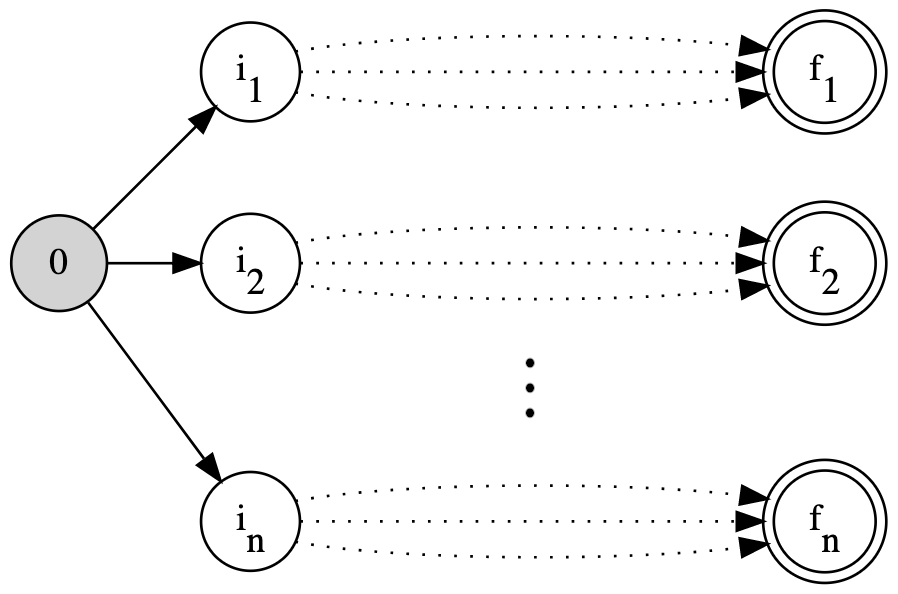
\includegraphics[
		height=5cm,
		keepaspectratio,
	  ]{img/fa-union.png}
	\caption{Краен автомат, получен от обединението на автоматите от лексическа граматика с n на брой правила.}
	\label{fig:FaUnion}
\end{figure}

\begin{example}
	Нека разгледаме следната спецификация:
	\begin{figure}[!htb]
		\begin{center}
			\begin{tabular}{ |l|l| } 
			\hline
			Token & Description \\
			\hline
			Id & \verb/[a-zA-Z_][a-zA-Z0-9_]*/ \\
			Number & \verb/[0-9]+(\.[0-9]+)?/ \\
			Boolean & \verb/true|false/ \\
			Operator & \verb/=|==|!=|<|<=|>|>=/ \\
			If & \verb/if/ \\
			Else & \verb/else/ \\
			Return & \verb/return/ \\
			BraceOpen & \verb/{/ \\
			BraceClose & \verb/}/\\
			WS & \verb/[ \t\r\n]+/ \\
			\hline
			\end{tabular}
		\end{center}
		\label{fig:Lexgr1}
		\caption{Лексическа граматика}
	\end{figure}

	\noindent Входният текст \emph{"num\textunderscore1=90.4"}, се разбива на следните лексеми: \\ (\emph{num\textunderscore1}, \textbf{Id}), (\emph{=}, \textbf{Operator}), (\emph{90.4}, \textbf{Number}).

	\noindent Друг пример е думата \emph{"if valid==true return 0"}, за която получаваме: \\ (\emph{if}, \textbf{If}), (\emph{' '}, \textbf{WS}), (\emph{valid}, \textbf{Id}), (\emph{==}, \textbf{Operator}), (\emph{true}, \textbf{Boolean}), (\emph{' '}, \textbf{WS}), \\ (\emph{return}, \textbf{Return}), (\emph{' '}, \textbf{WS}), (\emph{0}, \textbf{Number}).

	Всяко правило се представя чрез краен автомат, като на пример този за "Boolean" е изобразен на Фигура \ref{fig:Fa1}.

	\begin{figure}[!htb]
		\centering
		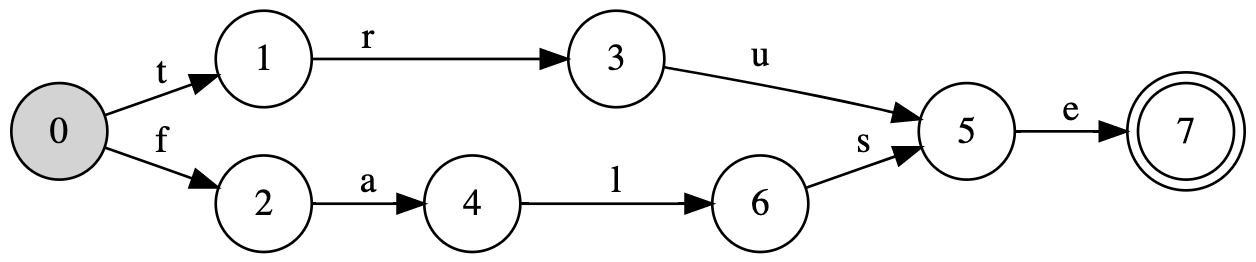
\includegraphics[
			width=12cm,
			keepaspectratio,
	  	]{img/fa1.png}
		\caption{Краен автомат разпознаващ думите \emph{true} или \emph{false}}
		\label{fig:Fa1}
	\end{figure}

	След като автоматите за всяко правило са построени, следващата стъпка е да се обединят в единствен краен автомат (Фигура \ref{fig:Fa3}), който се симулира по време на сканирането на входния текст.

	\begin{figure}[!htb]
		\centering
		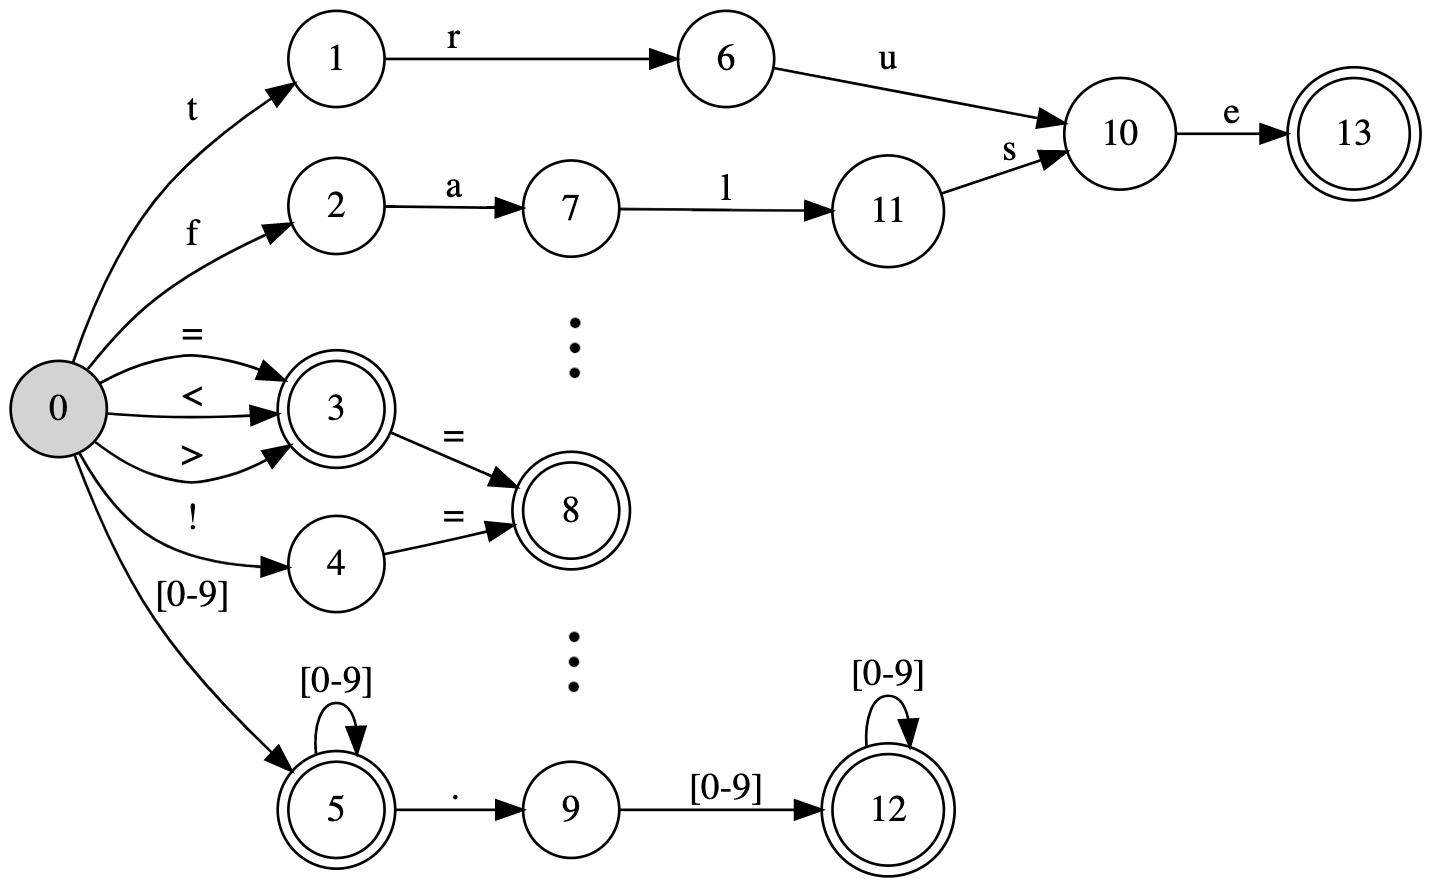
\includegraphics[
			width=16cm,
			height=8cm,
			keepaspectratio,
	  	]{img/fa3.png}
		\caption{Краен автомат, получен от обединението на автоматите от лексическата граматика. За яснота са изобразени само Boolean, Operator и Number.}
		\label{fig:Fa3}
	\end{figure}
	Нека разгледаме входния текст \emph{"1 > 0.99 == true"}. Преди да започнем да го четем, авоматът се намира в началното си състояние 0. Четем \emph{'1'} и преминаваме в състояние 5. Следващият символ е \emph{'>'}, за който няма преход. Намираме се във финално състояние на автомата на лексемата Number, съответно извеждаме (\emph{1}, \textbf{Number}) и се връщаме в началното състояние. Аналогично от 0 имаме преход с \emph{'>'}, който води до състояние 3, което е финално. Няма преход от 3 на \emph{'0'}, съответно извеждаме (\emph{>}, \textbf{Operator}) и се връщаме в 0. Прочитайки \emph{'0'}, автоматът преминава в състояние 5, което е финално, но следващият символ е \emph{'.'}, така че можем да продължим със симулацията като стигаме до състояние 12 и извеждаме (\emph{'0.99'}, \textbf{Number}). Аналогично по пътя 0,3,8 ще изведем (\emph{'=='}, \textbf{Operator}) и в последствие по 0,1,6,10,13 ще изведем (\emph{'true'}, \textbf{Boolean}), като с това сме изчерпали символите в тескта и процедурата приключва.
\end{example}

В определени случаи този подход може да се окаже неефективен. Нека разгледаме следния прост пример.

\begin{figure}[!htb]
	\begin{center}
		\begin{tabular}{ |l|l| } 
		\hline
		Token & Description \\
		\hline
		A & \verb/аа/ \\
		B & \verb/a+b/ \\
		\hline
		\end{tabular}
	\end{center}
	\centering
	\begingroup
		\tikzset{every picture/.style={scale=0.75}}%
		% Start of code
% \begin{tikzpicture}[anchor=mid,>=latex',line join=bevel,]
\begin{tikzpicture}[>=latex',line join=bevel,]
  \pgfsetlinewidth{1bp}
%%
\pgfsetcolor{black}
  % Edge: 0 -> 1
  \draw [->] (34.057bp,72.693bp) .. controls (44.705bp,78.84bp) and (59.198bp,87.207bp)  .. (80.188bp,99.325bp);
  \definecolor{strokecol}{rgb}{0.0,0.0,0.0};
  \pgfsetstrokecolor{strokecol}
  \draw (57.107bp,94.0bp) node {a};
  % Edge: 0 -> 3
  \draw [->] (34.057bp,55.702bp) .. controls (44.705bp,49.835bp) and (59.198bp,41.848bp)  .. (80.188bp,30.281bp);
  \draw (57.107bp,51.0bp) node {a};
  % Edge: 1 -> 2
  \draw [->] (114.39bp,108.0bp) .. controls (123.82bp,108.0bp) and (135.81bp,108.0bp)  .. (157.02bp,108.0bp);
  \draw (135.71bp,115.0bp) node {a};
  % Edge: 3 -> 3
  \draw [->] (89.48bp,39.037bp) .. controls (88.106bp,48.858bp) and (90.351bp,58.0bp)  .. (96.214bp,58.0bp) .. controls (99.878bp,58.0bp) and (102.13bp,54.429bp)  .. (102.95bp,39.037bp);
  \draw (96.214bp,65.0bp) node {a};
  % Edge: 3 -> 4
  \draw [->] (114.39bp,22.0bp) .. controls (123.82bp,22.0bp) and (135.81bp,22.0bp)  .. (157.02bp,22.0bp);
  \draw (135.71bp,29.0bp) node {b};
  % Node: 0
\begin{scope}
  \definecolor{strokecol}{rgb}{0.0,0.0,0.0};
  \pgfsetstrokecolor{strokecol}
  \definecolor{fillcol}{rgb}{0.83,0.83,0.83};
  \pgfsetfillcolor{fillcol}
  \filldraw [opacity=1] (18.0bp,64.0bp) ellipse (18.0bp and 18.0bp);
  \draw (18.0bp,64.0bp) node {0};
\end{scope}
  % Node: 1
\begin{scope}
  \definecolor{strokecol}{rgb}{0.0,0.0,0.0};
  \pgfsetstrokecolor{strokecol}
  \draw (96.21bp,108.0bp) ellipse (18.0bp and 18.0bp);
  \draw (96.214bp,108.0bp) node {1};
\end{scope}
  % Node: 3
\begin{scope}
  \definecolor{strokecol}{rgb}{0.0,0.0,0.0};
  \pgfsetstrokecolor{strokecol}
  \draw (96.21bp,22.0bp) ellipse (18.0bp and 18.0bp);
  \draw (96.214bp,22.0bp) node {3};
\end{scope}
  % Node: 2
\begin{scope}
  \definecolor{strokecol}{rgb}{0.0,0.0,0.0};
  \pgfsetstrokecolor{strokecol}
  \draw (179.21bp,108.0bp) ellipse (18.0bp and 18.0bp);
  \draw (179.21bp,108.0bp) ellipse (22.0bp and 22.0bp);
  \draw (179.21bp,108.0bp) node {2};
\end{scope}
  % Node: 4
\begin{scope}
  \definecolor{strokecol}{rgb}{0.0,0.0,0.0};
  \pgfsetstrokecolor{strokecol}
  \draw (179.21bp,22.0bp) ellipse (18.0bp and 18.0bp);
  \draw (179.21bp,22.0bp) ellipse (22.0bp and 22.0bp);
  \draw (179.21bp,22.0bp) node {4};
\end{scope}
%
\end{tikzpicture}
% End of code
	\endgroup
	\label{fig:Lexgr2}
	\caption{Лексическа граматика и построеният по нея краен автомат.}
\end{figure}

\begin{example}
	Граматиката на Фигура \ref{fig:Lexgr2} съдържа две правила. Правило \textbf{A} представлява единствено думата \emph{"aa"}. Правило \textbf{B} обхваща думите, съдържащи \emph{'a'} поне веднъж, които завършват с \emph{'b'} като на пример \emph{"ab", "aab", "aaab"} и т.н. Входният текст \emph{"aabaaaa} се разбива на следните лексеми: (\emph{'aab'}, \textbf{B}), (\emph{'aa'}, \textbf{A}), (\emph{'aa'}, \textbf{A}).

	Нека разгледаме случая, в който сканираме текста \emph{"aaaaaaaaаа"}, състоящ се от пет еднакви тоукъна - (\emph{'aa'}, \textbf{A}). Очевидно, за да изведем \textbf{А} е необходимо да сканираме текста до самия му край, за да се уверим, че не съществува \emph{'b'}. Това се случва за всеки изведен тоукън, което води до неоптимална сложност на процедурата от \( \mathcal{O}(n^2) \).
\end{example}

Лексическият анализ чрез бимашина се справя с този проблем като сканирането на текста се случва едновременно от ляво на дясно и от дясно на ляво, с което се гарантира линейно време на изпълнение. Целта на тази работа е да се представи конструкция на такава бимашина по зададена лексическа граматика и алгоритъм за осъществяване на лексическия анализ.

\pagebreak
\section{Основни дефиниции}

\subsection{Крайни автомати}

\begin{definition}
	\emph{Краен автомат} дефинираме като петорка \( \mathcal{A} = \langle \Sigma, Q, I, F, \Delta \rangle \), където

	\begin{itemize}
		\item \( \Sigma \) е \emph{крайна азбука от символи}
		\item \( Q \) е \emph{крайно множество от състояния}
		\item \( I \subseteq Q \) е \emph{множество от начални състояния}
		\item \( F \subseteq Q \) е \emph{множество от финални състояния}
		\item \( \Delta \subseteq Q \times \Sigma \times Q \) е \emph{релация на прехода}
	\end{itemize}
 
	Тройки от вида \( \langle q_1, m, q_2 \rangle \in \Delta \) наричаме \emph{преходи} и казваме, че започва състояние \( q_1 \), има етикет \( m \) и завършва в състояние \( q_2 \). Алтернативно, тези преходи обозначаваме като \( q_1 \to^m q_2 \).
\end{definition}

\begin{definition}  
	Нека \( \mathcal{A} \) е краен автомат. \emph{Разширена релация на прехода} \( \Delta^* \subseteq Q \times \Sigma^* \times Q \) дефинираме индуктивно:

	\begin{itemize}
		\item \( \langle q, \epsilon, q \rangle \in \Delta^* \) за всяко \( q \in Q \)
		\item \( \langle q_1, wa, q_2 \rangle \in \Delta^* \) за всяко \( q_1, q_2, q \in Q \), \( a \in \Sigma, w \in \Sigma^* \), ако \( \langle q_1, w, q \rangle \in \Delta^* \) и \( \langle q, a, q_2 \rangle \in \Delta \)
	\end{itemize}
\end{definition}

\begin{definition} 
	Нека \( \mathcal{A} = \langle \Sigma, Q, I, F, \Delta \rangle \) е краен автомат. \emph{Път} в \( \mathcal{A} \) наричаме крайна редица от преходи с дължина \( k > 0 \) 
	\[ \pi = q_0 \to^{a_1} q_1 \to^{a_2} \ldots \to^{a_k} q_k \] 
	където \( \langle q_{i-1}, a_i, q_i \rangle \in \Delta \) за \( i = 1 \ldots k \). Казваме, че \emph{пътят} започва от състояние \( q_0 \) и завършва в състояние \( q_k \). Елементите \( q_0,q_1, \ldots ,q_k \) наричаме \emph{състояния на пътя}, а думата \( w = a_1 a_2 \ldots a_k \) наричаме \emph{етикет на пътя}. \newline \emph{Успешен път} в автомата е \emph{път}, който започва от начално състояние и завършва във финално състояние.
\end{definition}

\begin{figure}[!htb]
	\centering
	% Start of code
% \begin{tikzpicture}[anchor=mid,>=latex',line join=bevel,]
\begin{tikzpicture}[>=latex',line join=bevel,]
  \pgfsetlinewidth{1bp}
%%
\pgfsetcolor{black}
  % Edge: 0 -> 1
  \draw [->] (41.38bp,33.346bp) .. controls (53.024bp,40.533bp) and (68.186bp,49.893bp)  .. (89.207bp,62.868bp);
  \definecolor{strokecol}{rgb}{0.0,0.0,0.0};
  \pgfsetstrokecolor{strokecol}
  \draw (65.5bp,56.0bp) node {b};
  % Edge: 0 -> 2
  \draw [->] (44.085bp,23.735bp) .. controls (64.334bp,25.44bp) and (95.778bp,28.188bp)  .. (123.0bp,31.0bp) .. controls (133.76bp,32.112bp) and (145.59bp,33.464bp)  .. (165.94bp,35.889bp);
  \draw (105.0bp,38.0bp) node {\(\epsilon\)};
  % Edge: 1 -> 1
  \draw [->] (98.266bp,89.037bp) .. controls (96.892bp,98.858bp) and (99.137bp,108.0bp)  .. (105.0bp,108.0bp) .. controls (108.66bp,108.0bp) and (110.92bp,104.43bp)  .. (111.73bp,89.037bp);
  \draw (105.0bp,115.0bp) node {a};
  % Edge: 1 -> 2
  \draw [->] (122.93bp,73.777bp) .. controls (130.82bp,73.967bp) and (140.18bp,73.252bp)  .. (148.0bp,70.0bp) .. controls (154.19bp,67.427bp) and (159.98bp,63.257bp)  .. (172.2bp,51.623bp);
  \draw (144.5bp,79.0bp) node {a};
  % Edge: 1 -> 2
  \draw [->] (120.65bp,62.769bp) .. controls (126.79bp,59.127bp) and (134.1bp,55.085bp)  .. (141.0bp,52.0bp) .. controls (145.96bp,49.782bp) and (151.38bp,47.722bp)  .. (166.36bp,42.716bp);
  \draw (144.5bp,59.0bp) node {b};
  % Edge: 2 -> 0
  \draw [->] (168.41bp,28.627bp) .. controls (156.67bp,21.673bp) and (139.47bp,12.77bp)  .. (123.0bp,9.0bp) .. controls (99.748bp,3.6755bp) and (72.92bp,7.7011bp)  .. (43.121bp,15.249bp);
  \draw (105.0bp,16.0bp) node {a};
  % Node: 0
\begin{scope}
  \definecolor{strokecol}{rgb}{0.0,0.0,0.0};
  \pgfsetstrokecolor{strokecol}
  \definecolor{fillcol}{rgb}{0.83,0.83,0.83};
  \pgfsetfillcolor{fillcol}
  \filldraw [opacity=1] (22.0bp,22.0bp) ellipse (18.0bp and 18.0bp);
  \draw (22.0bp,22.0bp) ellipse (22.0bp and 22.0bp);
  \draw (22.0bp,22.0bp) node {0};
\end{scope}
  % Node: 1
\begin{scope}
  \definecolor{strokecol}{rgb}{0.0,0.0,0.0};
  \pgfsetstrokecolor{strokecol}
  \draw (105.0bp,72.0bp) ellipse (18.0bp and 18.0bp);
  \draw (105.0bp,72.0bp) node {1};
\end{scope}
  % Node: 2
\begin{scope}
  \definecolor{strokecol}{rgb}{0.0,0.0,0.0};
  \pgfsetstrokecolor{strokecol}
  \draw (184.0bp,38.0bp) ellipse (18.0bp and 18.0bp);
  \draw (184.0bp,38.0bp) node {2};
\end{scope}
%
\end{tikzpicture}
% End of code

	\caption{Недетерминиран краен автомат}
	\label{fig:Nfa}
\end{figure}

\begin{example}
	Нека е зададена азбука \( \Sigma = \{ a,b,\epsilon \} \) и автомат \( \mathcal{A} \) над \( \Sigma \) със състояния \( Q = \{ 0, 1, 2 \} \), начални \( I = \{ 0 \} \), финални \( F = \{ 0 \} \) и релация на прехода 
	\[ \Delta = \{ \langle 0, b, 1 \rangle, \langle 0, \epsilon, 2 \rangle, \langle 1, a, 1 \rangle, \langle 1, a, 2 \rangle \, \langle 1, b, 2 \rangle, \langle 2, a, 0 \rangle \} \]
	\( \mathcal{A} \) е изобразен на Фигура \ref{fig:Nfa}. \( 0 \to^{b} 1 \to^{a} 1 \to^{b} 2 \to^{a} 0 \) е успешен път, разпознавайки думата \emph{baba}.
\end{example}

\begin{definition} 
	Нека \( \mathcal{A} \) е краен автомат. Множеството от етикети на всички успещни пътища в \( \mathcal{A} \) наричаме \emph{език на \( \mathcal{A} \)} и обозначаваме като \( L(\mathcal{A}) \). \[ L(\mathcal{A}) = \{ w \in \Sigma^* \mid \exists i \in I, f \in F : \langle i, w, f \rangle \in \Delta^* \} \]
\end{definition}

\begin{definition} 
	Нека \( \mathcal{A}_1 \) и \( \mathcal{A}_2 \) са крайни автомати. Казваме, че \( \mathcal{A}_1 \) е еквивалентен на \( \mathcal{A}_2 \) (\( \mathcal{A}_1 \equiv \mathcal{A}_2 \)), ако езиците им съвпадат (\( L(\mathcal{A}_1) = L(\mathcal{A}_2) \))
\end{definition}

\begin{definition}
	Kраен автомат \( \mathcal{A} = \langle \Sigma, Q, I, F, \Delta \rangle \) е \emph{детерминиран}, ако:

	\begin{itemize}
		\item \( \mathcal{A} \) има единствено начално състояние \(I = \{q_0\}\).
		\item За всяко \( q_1 \in Q \) и символ \( a \in \Sigma \), съществува не повече от едно \( q_2 \in Q \), такова че \( \langle q_1, a, q_2 \rangle \in \Delta \).
	\end{itemize} 

	\noindent Иначе казано, релацията на прехода може да се представи като частична функция \( \delta: Q \times \Sigma \to Q \) и \emph{детерминираните автомати} можем преставим в следния вид \[ \mathcal{A}_D = \langle \Sigma, Q, q_0, F, \delta \rangle \]

	Предимството на \emph{детерминираните автомати} се изразява в това, че могат да разпознават дали дума \( w \) принадлежи на езика на автомата \( L(\mathcal{A}_D) \) за линейно време спрямо дължината ѝ - \( O(|w|) \), но в определени случаи могат да имат експоненциален брой състояния спрямо еквивалентният им недетерминиран автомат.
\end{definition}

\begin{figure}[!htb]
	\centering
	% Start of code
% \begin{tikzpicture}[anchor=mid,>=latex',line join=bevel,]
\begin{tikzpicture}[>=latex',line join=bevel,]
  \pgfsetlinewidth{1bp}
%%
\pgfsetcolor{black}
  % Edge: 0 -> 0
  \draw [->] (14.317bp,42.991bp) .. controls (13.369bp,53.087bp) and (15.93bp,62.0bp)  .. (22.0bp,62.0bp) .. controls (25.889bp,62.0bp) and (28.337bp,58.342bp)  .. (29.683bp,42.991bp);
  \definecolor{strokecol}{rgb}{0.0,0.0,0.0};
  \pgfsetstrokecolor{strokecol}
  \draw (22.0bp,69.0bp) node {a};
  % Edge: 0 -> 1
  \draw [->] (43.022bp,29.416bp) .. controls (53.675bp,33.361bp) and (66.893bp,38.257bp)  .. (87.741bp,45.978bp);
  \draw (65.5bp,46.0bp) node {b};
  % Edge: 1 -> 2
  \draw [->] (119.63bp,62.906bp) .. controls (131.01bp,72.014bp) and (147.44bp,85.165bp)  .. (168.71bp,102.19bp);
  \draw (144.11bp,91.0bp) node {a};
  % Edge: 1 -> 3
  \draw [->] (123.04bp,52.0bp) .. controls (150.43bp,52.0bp) and (204.51bp,52.0bp)  .. (247.82bp,52.0bp);
  \draw (183.21bp,59.0bp) node {b};
  % Edge: 2 -> 3
  \draw [->] (197.95bp,102.65bp) .. controls (210.29bp,93.363bp) and (228.62bp,79.56bp)  .. (251.41bp,62.399bp);
  \draw (222.71bp,93.0bp) node {b};
  % Edge: 2 -> 4
  \draw [->] (197.25bp,124.43bp) .. controls (203.47bp,129.19bp) and (211.28bp,134.25bp)  .. (219.21bp,137.0bp) .. controls (223.88bp,138.62bp) and (228.98bp,139.63bp)  .. (244.14bp,140.96bp);
  \draw (222.71bp,145.0bp) node {a};
  % Edge: 3 -> 0
  \draw [->] (248.27bp,47.884bp) .. controls (221.74bp,41.645bp) and (168.72bp,29.994bp)  .. (123.0bp,25.0bp) .. controls (100.13bp,22.501bp) and (74.15bp,21.785bp)  .. (44.136bp,21.67bp);
  \draw (144.11bp,36.0bp) node {a};
  % Edge: 4 -> 2
  \draw [->] (247.16bp,128.57bp) .. controls (240.77bp,124.99bp) and (233.37bp,121.36bp)  .. (226.21bp,119.0bp) .. controls (221.48bp,117.44bp) and (216.31bp,116.29bp)  .. (201.28bp,114.07bp);
  \draw (222.71bp,126.0bp) node {b};
  % Edge: 4 -> 4
  \draw [->] (258.53bp,160.99bp) .. controls (257.58bp,171.09bp) and (260.14bp,180.0bp)  .. (266.21bp,180.0bp) .. controls (270.1bp,180.0bp) and (272.55bp,176.34bp)  .. (273.9bp,160.99bp);
  \draw (266.21bp,187.0bp) node {a};
  % Node: 0
\begin{scope}
  \definecolor{strokecol}{rgb}{0.0,0.0,0.0};
  \pgfsetstrokecolor{strokecol}
  \definecolor{fillcol}{rgb}{0.83,0.83,0.83};
  \pgfsetfillcolor{fillcol}
  \filldraw [opacity=1] (22.0bp,22.0bp) ellipse (18.0bp and 18.0bp);
  \draw (22.0bp,22.0bp) ellipse (22.0bp and 22.0bp);
  \draw (22.0bp,22.0bp) node {0};
\end{scope}
  % Node: 1
\begin{scope}
  \definecolor{strokecol}{rgb}{0.0,0.0,0.0};
  \pgfsetstrokecolor{strokecol}
  \draw (105.0bp,52.0bp) ellipse (18.0bp and 18.0bp);
  \draw (105.0bp,52.0bp) node {1};
\end{scope}
  % Node: 2
\begin{scope}
  \definecolor{strokecol}{rgb}{0.0,0.0,0.0};
  \pgfsetstrokecolor{strokecol}
  \draw (183.21bp,113.0bp) ellipse (18.0bp and 18.0bp);
  \draw (183.21bp,113.0bp) node {2};
\end{scope}
  % Node: 3
\begin{scope}
  \definecolor{strokecol}{rgb}{0.0,0.0,0.0};
  \pgfsetstrokecolor{strokecol}
  \draw (266.21bp,52.0bp) ellipse (18.0bp and 18.0bp);
  \draw (266.21bp,52.0bp) node {3};
\end{scope}
  % Node: 4
\begin{scope}
  \definecolor{strokecol}{rgb}{0.0,0.0,0.0};
  \pgfsetstrokecolor{strokecol}
  \draw (266.21bp,140.0bp) ellipse (18.0bp and 18.0bp);
  \draw (266.21bp,140.0bp) ellipse (22.0bp and 22.0bp);
  \draw (266.21bp,140.0bp) node {4};
\end{scope}
%
\end{tikzpicture}
% End of code

	\caption{Детерминиран краен автомат}
\end{figure}

\begin{definition}
	Нека \( \mathcal{A}_D = \langle \Sigma, Q, q_0, F, \delta \rangle \) е \emph{детерминиран краен автомат}. \emph{Разширена функция на прехода} \( \delta^*: Q \times \Sigma^* \to Q \) дефинираме индуктивно:

	\begin{itemize}
		\item \( \delta^*(q, \epsilon) = q \)
		\item \( \delta^*(q, aw) = \delta^*(\delta(q, a), w) \), където \( a \in \Sigma, w \in \Sigma^* \)
	\end{itemize}
\end{definition}

\begin{theorem}
	За всеки краен автомат \(\mathcal{A} = \langle \Sigma, Q, I, F, \Delta \rangle \), съществува еквивалентен на него, детерминиран краен автомат \( \mathcal{A}_D \), където \( L(\mathcal{A}) = L(\mathcal{A}_D) \).
	\begin{proof}
		Нека \( \mathcal{A} \) е краен автомат, на който сме премахнали \( \epsilon \)-преходите. Строим \emph{детерминиран краен автомат} \( \mathcal{A}_D = \langle \Sigma, 2^Q, I, F_D, \delta \rangle \), където:
		\begin{itemize}
			\item \( F_D = \{ S \in 2^Q \mid S \cap F \neq \emptyset \} \)
			\item \( \delta(S,a) = \{ q \in Q \mid \exists p \in S : \langle p, a, q \rangle \in \Delta \} \)
		\end{itemize}
		С индукция по дължината на \( w \), ще покажем, че за произволна дума \( w \in \Sigma^* \) твръденията \( \exists i \in I: \langle i, w, p \rangle \in \Delta^* \) и \( p \in \delta^*(I, w)\) са еквивалентни:
		\begin{itemize}
			\item \emph{База}: за \( |w| = 0 \) имаме \( w = \epsilon \). Тогава \( \exists i \in I: \langle  i, \epsilon, i \rangle \in \Delta^* \). Тъй като \( \mathcal{A} \) няма \( \epsilon \)-преходи, то \( \delta^*(I, \epsilon) = I \).
			
			\item \emph{Индукция}: \( w = w'a, a \in \Sigma, |w| = |w'| + 1 \). \newline
			\( (\Rightarrow) \) Нека допуснем, че \( \exists i \in I \), така че \( \langle i, w'a, p \rangle \in \Delta^* \), което значи, че \( \exists p' \in Q: \langle p', a, p \rangle \in \Delta \). По индуктивното предположение знаем, че и \( p' \in \delta^*(I, w') \) и от дефиницията на \( \delta \) следва, че \( p \in \delta(\delta^*(I, w'), a) \). \newline
			\( (\Leftarrow) \) Нека допуснем, че \( p \in \delta^*(I, w'a) \). Тогава \( \exists p': p' \in \delta^*(I, w') \). От индуктиното предположение знаем, че \( \langle i, w', p' \rangle \in \Delta^* \) и от дефинициите на \( \delta  \) и \( \Delta \) следва, че \( \langle p', a, p \rangle \in \Delta \), от където следва, че \( \exists i \in I: \langle i, w'a, p \rangle \in \Delta^* \).
		\end{itemize}
		Така можем да заключим, че за всяка дума \( w \in L(\mathcal{A}) \), \( \exists i \in I, \exists f \in F : \langle i, w, f \rangle \in \Delta^* \) е изпълнено, че \( \delta^*(I, w) \in F_D \), следователно \( w \in L(\mathcal{A}_D) \) и \( L(\mathcal{A}) = L(\mathcal{A}_D) \).
	\end{proof}
\end{theorem}

\subsection{Крайни преобразуватели}

\begin{definition}
	\emph{Краен преобразувател} дефинираме като петорка \( \mathcal{T} = \langle \Sigma_1^* \times \Sigma_2^*, Q, I, F, \Delta \rangle \), където

	\begin{itemize}
		\item \( \Sigma_1, \Sigma_2 \) са \emph{крайни азбуки от символи}
		\item \( Q \) е \emph{крайно множество от състояния}
		\item \( I \subseteq Q \) е \emph{множество от начални състояния}
		\item \( F \subseteq Q \) е \emph{множество от финални състояния}
		\item \( \Delta \subseteq Q \times (\Sigma_1^* \times \Sigma_2^*) \times Q \) е \emph{релация на прехода}
	\end{itemize}
 
	Тройки от вида \( \langle q_1, \langle w, m \rangle, q_2 \rangle \in \Delta \) наричаме \emph{преходи} и казваме, че започва състояние \( q_1 \), има етикет по горната лента \( w \) и по долната лента \( m \) и завършва в състояние \( q_2 \). Алтернативно, тези преходи обозначаваме като \( q_1 \to^w_m q_2 \).
\end{definition}

\begin{definition} 
	Нека \( \mathcal{T} = \langle \Sigma_1^* \times \Sigma_2^*, Q, I, F, \Delta \rangle \) е краен преобразувател. \emph{Път} в \( \mathcal{T} \) наричаме крайна редица от преходи с дължина \( k > 0 \) 
	\[ \pi = q_0 \to^{w_1}_{m_1} q_1 \to^{w_2}_{m_2} \ldots \to^{w_k}_{m_k}  q_k \] 
	където \( \langle q_{i-1}, \langle w_i, m_i \rangle, q_i \rangle \in \Delta \) за \( i = 1 \ldots k \). Казваме, че \emph{пътят} започва от състояние \( q_0 \) и завършва в състояние \( q_k \). Елементите \( q_0,q_1, \ldots ,q_k \) наричаме \emph{състояния на пътя}, а думата \( w = w_1 w_2 \ldots w_k \) наричаме \emph{входна дума} на пътя, а \( m = m_1 m_2 \ldots m_k \) е \emph{изходна дума} на пътя. \newline \emph{Успешен път} в преобразувателя започва от начално състояние и завършва във финално състояние.
\end{definition}

\begin{figure}[!htb]
	\centering
	% Start of code
% \begin{tikzpicture}[anchor=mid,>=latex',line join=bevel,]
\begin{tikzpicture}[>=latex',line join=bevel,]
  \pgfsetlinewidth{1bp}
%%
\pgfsetcolor{black}
  % Edge: 0 -> 1
  \draw [->] (36.835bp,66.461bp) .. controls (43.628bp,73.272bp) and (52.411bp,80.407bp)  .. (62.0bp,84.0bp) .. controls (70.197bp,87.071bp) and (79.618bp,87.58bp)  .. (98.159bp,85.873bp);
  \definecolor{strokecol}{rgb}{0.0,0.0,0.0};
  \pgfsetstrokecolor{strokecol}
  \draw (70.945bp,94.0bp) node {a/d};
  % Edge: 0 -> 2
  \draw [->] (42.234bp,41.004bp) .. controls (48.469bp,38.253bp) and (55.463bp,35.34bp)  .. (62.0bp,33.0bp) .. controls (70.433bp,29.982bp) and (79.79bp,27.161bp)  .. (98.033bp,22.16bp);
  \draw (70.945bp,40.0bp) node {b/d};
  % Edge: 1 -> 0
  \draw [->] (99.425bp,74.306bp) .. controls (93.413bp,71.481bp) and (86.413bp,68.392bp)  .. (79.89bp,66.0bp) .. controls (71.374bp,62.877bp) and (61.955bp,60.003bp)  .. (43.517bp,54.95bp);
  \draw (70.945bp,73.0bp) node {b/\(\epsilon\)};
  % Edge: 2 -> 0
  \draw [->] (99.067bp,10.797bp) .. controls (88.259bp,6.9443bp) and (73.813bp,3.9331bp)  .. (62.0bp,9.0bp) .. controls (54.255bp,12.322bp) and (47.322bp,18.021bp)  .. (34.816bp,31.943bp);
  \draw (70.945bp,16.0bp) node {c/\(\epsilon\)};
  % Node: 0
\begin{scope}
  \definecolor{strokecol}{rgb}{0.0,0.0,0.0};
  \pgfsetstrokecolor{strokecol}
  \definecolor{fillcol}{rgb}{0.83,0.83,0.83};
  \pgfsetfillcolor{fillcol}
  \filldraw [opacity=1] (22.0bp,50.0bp) ellipse (18.0bp and 18.0bp);
  \draw (22.0bp,50.0bp) ellipse (22.0bp and 22.0bp);
  \draw (22.0bp,50.0bp) node {0};
\end{scope}
  % Node: 1
\begin{scope}
  \definecolor{strokecol}{rgb}{0.0,0.0,0.0};
  \pgfsetstrokecolor{strokecol}
  \draw (115.89bp,82.0bp) ellipse (18.0bp and 18.0bp);
  \draw (115.89bp,82.0bp) node {1};
\end{scope}
  % Node: 2
\begin{scope}
  \definecolor{strokecol}{rgb}{0.0,0.0,0.0};
  \pgfsetstrokecolor{strokecol}
  \draw (115.89bp,18.0bp) ellipse (18.0bp and 18.0bp);
  \draw (115.89bp,18.0bp) node {2};
\end{scope}
%
\end{tikzpicture}
% End of code

	\caption{Краен преобразувател}
	\label{fig:Fst}
\end{figure}

\begin{example}
	Нека са зададени азбукаи \( \Sigma_1 = \{ a,b,c \}, \Sigma_2 = \{ d,\epsilon \} \) и преобразувател \( \mathcal{T} \) над \( \Sigma_1^* \times \Sigma_2^*\) със състояния \( Q = \{ 0, 1, 2 \} \), начални \( I = \{ 0 \} \), финални \( F = \{ 0 \} \) и релация на прехода \( \Delta = \{ \langle 0, \langle a, d \rangle, 1 \rangle, \langle 1, \langle b, \epsilon \rangle, 0 \rangle, \langle 0, \langle b, d \rangle, 2 \rangle, \langle 2, \langle c, \epsilon \rangle, 0 \rangle \} \). \newline
	\( \mathcal{T} \) е изобразен на Фигура \ref{fig:Fst}. \newline
	\( 0 \to^{b}_{d} 2 \to^{c}_{\epsilon} 0 \to^{a}_{d} 1 \to^{b}_{\epsilon} 0 \) е успешен път, превеждайки думата \emph{bcab} в \emph{dd}.
\end{example}

\begin{definition}
	Нека \( \mathcal{T} = \langle \Sigma_1^* \times \Sigma_2^*, Q, I, F, \Delta \rangle \) е краен преобразувател. \emph{Подлежащ автомат} на \( \mathcal{T} \) дефинираме като \( \mathcal{A} = \langle \Sigma, Q, I, F, \Delta' \rangle \), където \( \Delta' = \{ \langle p, w, q \rangle \mid \langle p, \langle w, m \rangle, q \rangle \in \Delta \}\)
\end{definition}

\subsection{Регулярни езици и релации}

\begin{definition} 
	\emph{Регулярен език} е множество над крайна азбука \( \Sigma \), което дефинираме индуктивно:
	\begin{itemize}
		\item \( \emptyset \) е регулярен език.
		\item ако \( a \in \Sigma \), то \( \{ a \} \) е регулярен език.
		\item ако \( L_1, L_2 \subseteq \Sigma^* \) са регулярни езици, то 
		\begin{itemize}
			\item \( L_1 \cup L_2 \) (обедниение)
			\item \( L_1 \cdot L_2 = \{ a \cdot b \mid a \in L_1, b \in L_2 \} \) (конкатенация)
			\item \( L_1^* = \bigcup_{i=0}^{\infty}L^i \) (звезда на Клини)
		\end{itemize}
		 са също регулярни езици.
		\item Не съществуват други регулярни езици.
	\end{itemize}
	Регулярните езици са също така \emph{затворени} относно операциите \emph{допълнение} (\( \Sigma^* \setminus L_1 \)), \emph{разлика} (\( L_1 \setminus L_2 \)), \emph{обръщане} (\( L_1^{-1} \)) и \emph{сечение} (\( L_1 \cap L_2 \)).
\end{definition}

\begin{definition} 
	\emph{Двоична регулярна стрингова релация} дефинираме индуктивно като множество от двойки над крайни азбуки \( \Sigma_1, \Sigma_2 \):
	\begin{itemize}
		\item \( \emptyset \) е регулярна релация.
		\item Ако \( a \in \Sigma_1 \times \Sigma_2 \), то \( \{ a \} \) е регулярна релация.
		\item Ако \( R_1, R_2 \) са регулярни релации, то:
		\begin{itemize}
			\item \( R_1 \cup R_2 \) (обединение)
			\item \( R_1 \cdot R_2 = \{ a \cdot b \mid a \in R_1, b \in R_2 \} \) (конкатенация)
			\item \( R_1^* = \bigcup_{i=0}^{\infty}R^i \) (звезда на Клини)
		\end{itemize}
		са също регулярни релации.
		\item Не съществуват други регулярни релации.
	\end{itemize}
\end{definition}

\begin{definition}
	Нека \( R_1, R_2, \in \Sigma^* \times \Sigma^* \) са \emph{двоични стрингови релации}. \emph{Конкатенацията} на \( R_1 \) и \( R_2 \) дефинираме както следва
	\[ R_1 \cdot R_2 = \{ \langle u_1 \cdot v_1, u_2 \cdot v_2 \rangle \mid \langle u_1, u_2 \rangle \in R_1, \langle v_1, v_2 \rangle \in R_2 \} \]
\end{definition}

\begin{definition} 
	\emph{Регулярен израз} наричаме дума над крайна азбука \( \Sigma \cup \{ (, ), \vert, * \} \)
	\begin{itemize}
		\item \( \epsilon \) е регулярен израз.
		\item Ако \( a \in \Sigma \), то \( a \) е регулярен израз.
		\item Ако \( E_1, E_2 \) са регулярни изрази, то \( E_1 | E_2 \) и \( E_1 E_2 \), \( E_1^* \) също са регулярни изрази.
		\item Не съществуват други регулярни изрази.
	\end{itemize}
	Всеки регулярен израз има сътветстващ регулярен език:
	\begin{itemize}
		\item \( L(\epsilon) = \emptyset \)
		\item \( L(a) = \{ a \}, a \in \Sigma \)
		\item \( L(E_1 | E_2) = L(E_1) \cup L(E_2) \)
		\item \( L(E_1 E_2) = L(E_1) \cdot L(E_2) \)
		\item \( L(E_1^*) = L(E_1)^* \)
	\end{itemize}
\end{definition}

\begin{example}
	\verb/(a|b)*c/ е \emph{регулярен израз}, разпознаващ думите \emph{c, ac, bc, aac, abc, abbc, bababbc ...}
\end{example}

\begin{theorem}{\emph{(Клини)}}
	За всеки регулярен израз \( E \) съществува краен автомат \( \mathcal{A} \), за който \( L(E) = L(\mathcal{A})\).
\end{theorem}

\begin{theorem}
	Всяка двоична регулярна стрингова релация може да се представи, чрез класически краен преобразувател.
\end{theorem}

\begin{example}
	\( R = \{ \langle ab, d \rangle, \langle bc, d \rangle \}^* \) е \emph{регулярна релация}, която е представена чрез чрез крайния преобразувател \(\mathcal{T}\) на Фигура \ref{fig:Fst}. \newline
	С \emph{dom(R)} бележим домейна на \(R\), който изразяваме чрез \emph{подлежащия автомат} на \( \mathcal{T} \), \( dom(R) =  \{ ab, bc, abab, abbc, bcab \dots \} \). С \emph{range(R)} обозначаваме кодомейна на релацията \( range(R) =  \{ \epsilon, d, dd, ddd, dddd \dots \} \).
\end{example}

\begin{example}
	Нека \(L\) е \emph{регулярен език}. \( Id(L) = \{ \langle w, w \rangle \mid w \in L \}\) е \emph{регулярна релация}.
\end{example}

\begin{definition}
	\emph{Регулярна стрнгова функция} наричаме регулярна стрингова релация, която е частична функция. 
\end{definition}

\subsection{Бимашини}

\begin{definition}
	 \emph{Класическа бимашина} дефинираме като тройка \( \mathcal{B} = \langle \mathcal{A}_L, \mathcal{A}_R, \psi \rangle \), където

	\begin{itemize}
		\item \( \mathcal{A}_L = \langle \Sigma, Q_L, s_L, Q_L, \delta_L \rangle \) и \( \mathcal{A}_R = \langle \Sigma, Q_R, s_R, Q_R, \delta_R \rangle \) са \emph{детерминирани крайни автомати} и ги наричаме съответно \emph{ляв и десен автомат} на бимашината. Всички състояния на тези автомати са финални.
		\item \( \psi:(Q_L \times \Sigma \times Q_R) \to \Sigma^* \) e частична функция, която наричаме \emph{изходна функция}.
	\end{itemize}
\end{definition}

\begin{definition} 
	Нека \( \mathcal{B} = \langle \mathcal{A}_L, \mathcal{A}_R, \psi \rangle \) е класическа бимашина, \( \Sigma \) е азбуката на на автоматите \( \mathcal{A}_L \) и \( \mathcal{A}_R \) и \( w = a_1a_2 \dots a_k \in \Sigma^* \) \( (k \geq 0) \) е дума и \( a_i \in \Sigma \) \( (1 \leq i \leq k) \) са букви. Ако \( \delta_L^*(a_1a_2 \ldots a_k) \) и \( \delta_R^*(a_ka_{k-1} \dots a_1) \) са дефинирани, то можем да получим двата пътя:
	\[ \pi_L = l_0 \to^{a_1} l_1 \to^{a_2} \ldots l_{k-1} \to^{a_k} l_k \]
	\[ \pi_R = r_0 \leftarrow^{a_1} r_1 \leftarrow^{a_2} \ldots r_{k-1} \leftarrow^{a_k} r_k \]
	Където \( \pi_L \) и \( \pi_R \) са пътища в съответно левия и десния автомат и думата \( w \) се разпознава от \( \mathcal{A}_L \) в посока от ляво на дясно, а от \( \mathcal{A}_R \), съответно от дясно на ляво. Ако за всички тройки \( \langle l_{i-1}, a_i, r_i \rangle \), изходната функция \( \psi(l_{i-1}, a_i, r_i) \) е дефинирана, то двойката пътища \( \langle \pi_L, \pi_R \rangle \) наричаме \emph{успешно изпълнение} на \( \mathcal{B} \) с етикет \( w = a_1a_2 \dots a_k \) и \emph{изход}
	\[ \mathcal{O_B}(w) = \psi(l_0, a_1, r_1) \cdot \psi(l_1, a_2, r_2) \cdot \dots \cdot \psi(l_{k-1}, a_k, r_k) \]
	\( \mathcal{O_B} \) наричаме \emph{изходна функция на бимашината} и казваме, че бимашината \emph{превежда} \(w\) в \(m\), ако \( \mathcal{O_B}(w) = m \), където \(m\) е резултат от конкатенацията на всички \( \psi(l_{i-1}, a_i, r_i) \) \( (1 \leq i \leq k) \).
\end{definition}

\noindent Бимашината чете входната дума и за всеки символ извежда дума над азбуката си. На всяка стъпка изведената от изходната функция \( \psi \) дума зависи от входния символ и двете състояния в които биха преминали левият и десният автомат, четейки входа съответно от ляво на дястно и от дясно на ляво. Крайният резултат е конкатенацията на всички така изведени думи.

\begin{definition}
	Нека \( \mathcal{B} = \langle \mathcal{A}_L, \mathcal{A}_R, \psi \rangle \) е бимашина. \emph{Разширената изходна функция \( \psi^* \)} дефинираме индуктивно:

	\begin{itemize}
		\item \( \psi^*(l, \epsilon, r) = \epsilon \) за всяко \( l \in Q_L, r \in Q_R \)
		\item \( \psi^*(l, wa, r) = \psi^*(l, w, \delta_R(r, a)) \cdot \psi(\delta^*_L(l, w), a, r) \), за \( l \in Q_L, r \in Q_R, w \in \Sigma^*, a \in \Sigma \)
	\end{itemize}
\end{definition}

\begin{figure}[!htb]
	\centering
	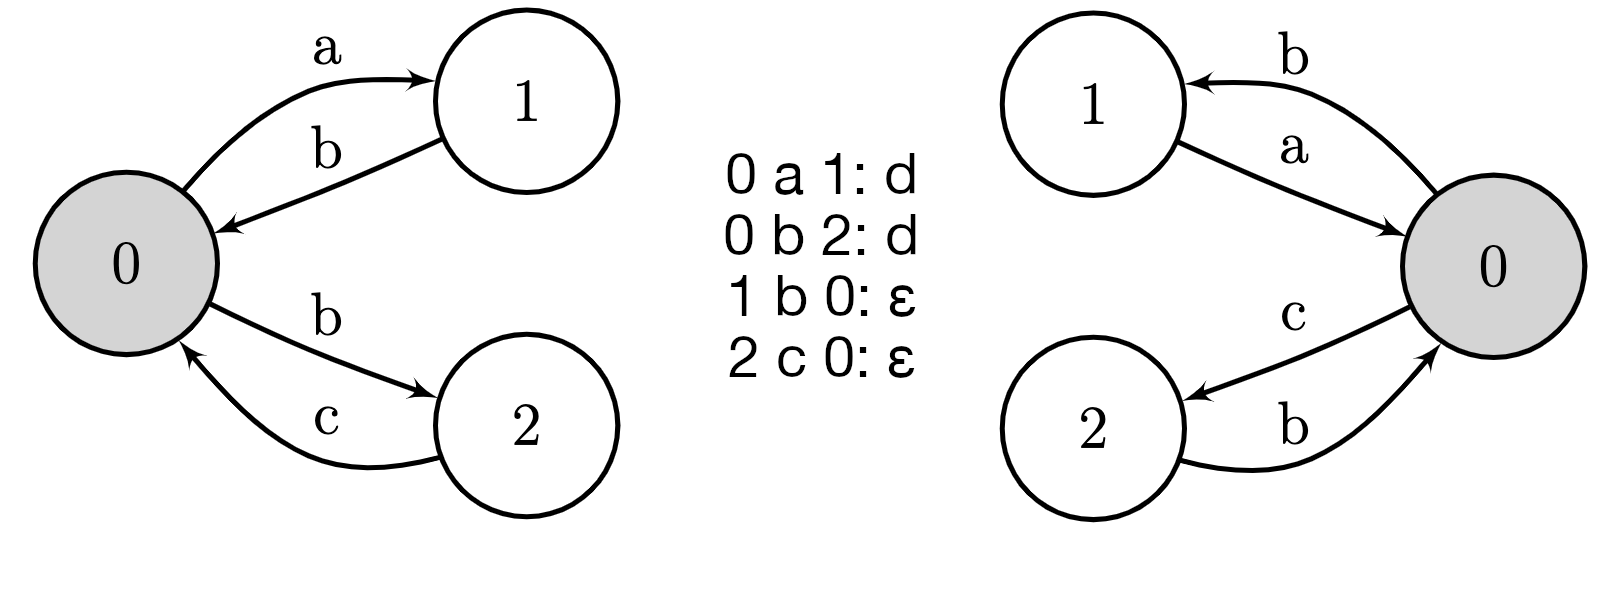
\includegraphics[
		width=12cm,
		height=6cm,
		keepaspectratio,
	  ]{img/bm.png}
	\caption{Бимашина представяща \( \{ \langle ab, d \rangle, \langle bc, d \rangle \}^* \)}
	\label{fig:Bm}
\end{figure}

\begin{example}{\emph{(Бимашина и изпълнение)}}
	Нека разлгледаме бимашината на Фигура \ref{fig:Bm}. Задаваме входна дума \emph{bcabbc}, което води до следното изпълнение на левия и десния автомат съответно.

	\[ \pi_L = 0 \to^{b} 2 \to^{c} 0 \to^{a} 1 \to^b 0 \to^{b} 2 \to^{c} 0 \]
	\[ \pi_R = 0 \leftarrow^{b} 2 \leftarrow^{c} 0 \leftarrow^{a} 1 \leftarrow^{b} 0 \leftarrow^{b} 2 \leftarrow^{c} 0 \]

	Изходната функция на бимашината \(\mathcal{O_B} \) прилагаме както следва:
	\[
		\psi(0,b,2) \cdot \psi(2,c,0) \cdot \psi(0,a,1) \cdot \psi(1,b,0) \cdot \psi(0,b,2) \cdot \psi(2,c,0) =
	d \cdot \epsilon \cdot d \cdot \epsilon \cdot d \cdot \epsilon = ddd
	\]

\end{example}

\begin{definition}
	Бимашина \( \mathcal{B} = \langle \mathcal{A}_L, \mathcal{A}_R, \psi \rangle \) наричаме \emph{тотална}, ако функциите на прехода \( \delta_L: Q_L \times \Sigma \to Q_L \) и \( \delta_R: Q_R \times \Sigma \to Q_R \) на левия и десния автомат съответно, както и функцията на изхода \( \psi: (Q_L \times \Sigma \times Q_R) \to \Sigma^* \) са \emph{тотални}.
\end{definition}

\begin{theorem}
	Класическите бимашини са еквивалентни по изразителност на регулярните функции. \cite{Schutzenberger:61}
\end{theorem}

\pagebreak
\section{Правила за заместване}

За двоичните стрингови релации можем да си мислим като множество от преводи, като на пример за двойката \( \langle u, v \rangle \) казваме, че думата \( u \) се превежда като \( v \).

\begin{definition}
	\emph{Правило за заместване} представяме във вида
	\[ E \to \beta \]
	където \( E \) е регулярен израз над крайна азбука \( \Sigma \), а \( \beta \in \Sigma^* \) е дума.
	\emph{Приложение на правилото върху текст} \( t \in \Sigma^* \) представлява заместването на поднизовете на \( t \), които са в езика \( L(E) \) с \( \beta \).
\end{definition}

\begin{figure}[!htb]
	\centering
	\begin{tikzpicture}
		\node[font=\Large] {
			\( a_1a_2 \dots a_i \dots a_{i+k} \dots a_{j} \dots a_{j+l} \dots a_n \)
		};
		\draw [decorate,decoration={brace,amplitude=5pt,raise=0pt},yshift=0pt]
		(-2.75,0.4) -- (-0.25,0.4) node [black,midway,xshift=0cm,yshift=0.5cm] {\footnotesize $ \in L(E) $};
		\draw [decorate,decoration={brace,amplitude=5pt,mirror,raise=0pt},yshift=0pt]
		(-2.75,-0.3) -- (-0.25,-0.3) node [black,midway,xshift=0cm,yshift=-0.5cm] {\footnotesize $ \beta $};
		\draw [decorate,decoration={brace,amplitude=5pt,raise=0pt},yshift=0pt]
		(0.8,0.4) -- (3.15,0.4) node [black,midway,xshift=0cm,yshift=0.5cm] {\footnotesize $ \in L(E) $};
		\draw [decorate,decoration={brace,amplitude=5pt,mirror,raise=0pt},yshift=0pt]
		(0.8,-0.3) -- (3.15,-0.3) node [black,midway,xshift=0cm,yshift=-0.5cm] {\footnotesize $ \beta $};
	\end{tikzpicture}
	\caption{Приложение на правило на заместване}
\end{figure}

\noindent \emph{Правила за заместване} можем да представим като \emph{регулярни стрингови релации}, използвайки единствено алгебрата на регулярните езици и релации. Те се реализират програмно чрез крайни преобразуватели. \cite{Kaplan&Kay:94}

\begin{definition}
	Нека разгледаме текст \( t \in \Sigma^* \). \emph{Kонтекст на заместване} наричаме тройка \( \langle u,v,w \rangle \), където \( t = uvw \). Също така \( u \) и \( w \) наричаме съответно \emph{префикс} и \emph{суфикс} на контекста, докато \( v \) наричаме \emph{фокус}.
\end{definition}

\begin{example}
	Нека разгледаме правилото \verb/ab|bc/ \( \to d \). След приложението му над текста \emph{abb}, ще получим \emph{db}, като \( \langle \epsilon, ab, b \rangle \) е единственият контекст на заместване. Приложението на правилото над \emph{abbacbca} ще доведе до \emph{dbacda} с два контекста на заместване \( \langle \epsilon, ab, bacbca \rangle \) и \( \langle abbac, bc, a \rangle \).
\end{example}

\subsection{Разрешаване на многозначности}

При прилагане на правило за заместване могат да възникнат многозначности в случаите, в които два контекста имат застъпващи се фокуси.

\begin{definition}
	Два контекста на заместване \( \langle u_1,v_1,w_1 \rangle \) и \( \langle u_2,v_2,w_2 \rangle \) за даден текст \( t \) \emph{се застъпват}, ако \( u_1 < u_2 < u_1v_1 \). Израза \( u_1 < u_2 \) четем като \( u_1 \) е \emph{префикс} на \( u_2 \).
\end{definition}

\begin{figure}[!htb]
	\centering
	\begin{tikzpicture}
	\draw (0,0) rectangle (3,1); % u_1
	\draw (0,0) rectangle (5,1); % u_2
	\draw[pattern=horizontal lines] (3,0) rectangle (7,1); % v_1
	\draw[pattern=vertical lines] (5,0) rectangle (8,1); % v_2
	\draw (7,0) rectangle (11,1); % w_1
	\draw (8,0) rectangle (11,1); % w_2
	\draw [decorate,decoration={brace,amplitude=10pt,raise=3pt},yshift=0pt]
		(0,1) -- (3,1) node [black,midway,xshift=0cm,yshift=0.75cm] {\footnotesize $u_1$};
	\draw [decorate,decoration={brace,amplitude=10pt,mirror,raise=3pt},yshift=0pt] 
		(0,0) -- (5,0) node [black,midway,xshift=0cm,yshift=-0.75cm] {\footnotesize $u_2$};
	\draw [decorate,decoration={brace,amplitude=10pt,raise=3pt},yshift=0pt]
		(3,1) -- (7,1) node [black,midway,xshift=0cm,yshift=0.75cm] {\footnotesize $v_1$};
	\draw [decorate,decoration={brace,amplitude=10pt,mirror,raise=3pt},yshift=0pt]
		(5,0) -- (8,0) node [black,midway,xshift=0cm,yshift=-0.75cm] {\footnotesize $v_2$};
	\draw [decorate,decoration={brace,amplitude=10pt,raise=3pt},yshift=0pt]
		(7,1) -- (11,1) node [black,midway,xshift=0cm,yshift=0.75cm] {\footnotesize $w_1$};
	\draw [decorate,decoration={brace,amplitude=10pt,mirror,raise=3pt},yshift=0pt]
		(8,0) -- (11,0) node [black,midway,xshift=0cm,yshift=-0.75cm] {\footnotesize $w_2$};
	\end{tikzpicture}
	\caption{Застъпващи се контексти}
\end{figure}

\begin{example}
	Нека разгледаме правилото \verb/ab|bc/ \( \to d \)) приложено над текста \( t = aabcb \). Получаваме контекстите \( \langle a, ab, cb \rangle \) и \( \langle aa, bc, b \rangle \), които очвевидно се застъпват и съответно стигаме до две различни валидни замествания \emph{adcb} и \emph{aadb}.
\end{example}

\begin{figure}[!htb]
	\centering
	\begin{tikzpicture}
	\draw (0,0) rectangle (3,1); % u_1
	\draw (0,0) rectangle (3,1); % u_2
	\draw[pattern=horizontal lines] (3,0) rectangle (8,1); % v_1
	\draw[pattern=vertical lines] (3,0) rectangle (6,1); % v_2
	\draw (8,0) rectangle (11,1); % w_1
	\draw (6,0) rectangle (11,1); % w_2
	\draw [decorate,decoration={brace,amplitude=10pt,raise=3pt},yshift=0pt]
		(0,1) -- (3,1) node [black,midway,xshift=0cm,yshift=0.75cm] {\footnotesize $u_1$};
	\draw [decorate,decoration={brace,amplitude=10pt,mirror,raise=3pt},yshift=0pt] 
		(0,0) -- (3,0) node [black,midway,xshift=0cm,yshift=-0.75cm] {\footnotesize $u_2$};
	\draw [decorate,decoration={brace,amplitude=10pt,raise=3pt},yshift=0pt]
		(3,1) -- (8,1) node [black,midway,xshift=0cm,yshift=0.75cm] {\footnotesize $v_1$};
	\draw [decorate,decoration={brace,amplitude=10pt,mirror,raise=3pt},yshift=0pt]
		(3,0) -- (6,0) node [black,midway,xshift=0cm,yshift=-0.75cm] {\footnotesize $v_2$};
	\draw [decorate,decoration={brace,amplitude=10pt,raise=3pt},yshift=0pt]
		(8,1) -- (11,1) node [black,midway,xshift=0cm,yshift=0.75cm] {\footnotesize $w_1$};
	\draw [decorate,decoration={brace,amplitude=10pt,mirror,raise=3pt},yshift=0pt]
		(6,0) -- (11,0) node [black,midway,xshift=0cm,yshift=-0.75cm] {\footnotesize $w_2$};
	\end{tikzpicture}
	\caption{Застъпващи се контексти с еднакво начало}
\end{figure}

\begin{example}
	Друг вид многозначност може да получим, когато фокусите на два контекста имат еднакво начало. Например, ако приложим правилото \(a+ \to d \) над тескт \( t = aa \), може получим превода \emph{dd}, на който отговарят контекстите \( \langle a, a, \epsilon \rangle \) и \( \langle \epsilon, a, a \rangle \), и \emph{d} с контекст \( \langle \epsilon, aa, \epsilon \rangle \).
\end{example}
%%
\begin{definition}
	Въвеждаме следните оператори над множества от контексти:
\[ AFTER(A, B) = \{ \langle u, v, w \rangle \in A \mid \forall \langle u', v', w' \rangle \in B : u' \cdot v' \leq u \land u' < u  \} \] 

\( AFTER \) избира измежду всички контексти в множеството \(A\) тези, в които фокусът \(v\) започва след всички фокуси в множеството \(B\).

\[ LEFTMOST(A) = \{ \langle u, v, w \rangle \in A \mid \forall \langle u', v', w' \rangle \in A : u \leq u' \} \]

\( LEFTMOST \) избира измежду всички контексти в \(A\), тези с чийто фокус се намира възможно най в ляво. Може да имаме повече от един такъв контекст.

\[ LONGEST(A) = \{ \langle u, v, w \rangle \in A \mid \forall \langle u', v', w' \rangle \in A : u \neq u' \lor v' \leq v \} \]

Измежду контекстите, чиито фокуси започват от една и съща позиция, \( LONGEST \) избира тези, които имат най-дълъг фокус.
\end{definition}

\begin{definition}
	Въвеждаме оператора \( LML(A) \) (leftmost-longest), чрез който ще елиминираме многозначностите. По дадено множество от контексти \(A\), \( LML(A) \) избира най-левите, най-дълги измежду тях.

	\[ LML(A) := \bigcup\limits_{i=0}^{\infty} C_{i} \]

	Където междинните множества \( C_i \) строим по индукция:

	\[ C_0 = \emptyset \]
	\[ C_{i+1} = C_i \cup LONGEST(LEFTMOST(AFTER(A, C_i))) \]

	\noindent \( LML(A) \) е крайно множество, защото \( A \) е крайно, т.е. след дадем момент редицата ще престане да нараства.
\end{definition}

\begin{proposition}
	Нека \( t \in \Sigma^* \) е текст и \(A\) е множество от контексти в \(t\). \( LML(A) \) съдържа само незастъпващи се контексти.

	\begin{proof}
		Нека \( LML(A) \) съдържа застъпващите се контексти \( \langle u_1, v_1, w_1 \rangle \) и \( \langle u_2, v_2, w_2 \rangle \) т.е. \( u_1 < u_2 < u_1v_1 \). Също така \( \langle u_1, v_1, w_1 \rangle \in C_{i_1} \) и \( \langle u_2, v_2, w_2 \rangle \in C_{i_2} \). Нека допуснем, че \( i_1 \geq i_2 \). В такъв случай:
		\[ \langle u_2, v_2, w_2 \rangle \in C_{i_2} = C_{i_2-1} \cup LONGEST(LEFTMOST(AFTER(A, C_{i_2-1}))) \]

		\noindent След като \( \langle u_2, v_2, w_2 \rangle \notin C_{i_2-1} \), то \( \langle u_2, v_2, w_2 \rangle \in LEFTMOST((AFTER(A, C_{i_2-1})) \).
		От допускането, че \( i_1 \geq i_2 \) следва, че \( \langle u_1, v_1, w_1 \rangle \in AFTER(A,C_{i_2-1}) \), което е в противоречие с дефиницията на \( LEFTMOST \) и следователно \( i_1 < i_2 \).

		\noindentСлед като \( i_1 < i_2 \), то \( \langle u_2, v_2, w_2 \rangle \notin C_i \) за \( i \leq i_1 \). При \( i > i_1 \), \( \langle u_1, v_1, w_1 \rangle \in C_i \), значи \( \langle u_2, v_2, w_2 \rangle \in AFTER(A, C_i) \), което не е възможно спрямо дефиницията на \( AFTER \) т.е. \( \langle u_2, v_2, w_2 \rangle \notin C_{i+1} \). Това противоречи с факта, че \( \langle u_2, v_2, w_2 \rangle \in C_{i_2} \) \( (i_1 < i_2) \), следователно \( LML(A) \) не съдържа застъпващи се контексти.
	\end{proof}
\end{proposition}

\begin{definition}
	Нека \( T \subseteq \Sigma^* \times \Sigma^* \) е релация и \( t \in \Sigma^* \) е текст. С \( A_{dom(T)} \) бележим множеството на всички поднизове в \(t\), които са в \(dom(T)\). Нека \[ t = u_1 v_1 x_2 v_2 \dots x_k v_k w_k \] е каноничното представяне на \(t\) за множеството \( LML(A_{dom(T)}) \). Тогава \(t'\) е \emph{заместването} на \(t\) с \(T\) под стратегията най-ляво-най-дълго срещане \[t = u_1 v_1' x_2 v_2' \dots x_k v_k' w_k\] и \( \langle v, v' \rangle \in T \) за \( 1 \leq i \leq k \). С \( R^{LML}(T) \) бележим релацията на заместване под стратегията най-ляво-най-дълго срещане за \(T\). Тя съдържа всички двойки \( \langle t, t' \rangle \in \Sigma^* \times \Sigma^* \), така че \( t' \) е заместване на \( t \) с \(T\) под стратегията най-ляво-най-дълго срещане.
\end{definition}

\begin{corollary}
	Нека \( T: \Sigma^+ \to \Sigma^* \) е функция, тогава релацията на заместване \( R^{LML}(T) \) е функционална.
\end{corollary}

\begin{example}
	Нека разгледаме правилото \verb/ab|bc/ \( \to d \) съответстващо на релацията \(T = \{ \langle ab,d \rangle, \langle bc, d \rangle \} \), приложено над текста \( t = aabcbab \). Получаваме контекстите \( \langle a, ab, cbab \rangle \), \( \langle aa, bc, bab \rangle \) и \( \langle aabcb, ab, \epsilon \rangle \). Очевидно първите два се застъпват, но стратегията най-ляво-най-дълго срещане определя първият и третият за валидни. Резултатът от заместането е \( R^{LML}(T)(aabcbab) = adcbd \).
\end{example}

\pagebreak
\section{Регулярни релации за лексически анализ}

 За да разбием даден текст на редица от тоукъни, е нужно да представим тези тоукъни под формата на регулярни изрази. Това представяне наричаме \emph{лексическа граматика}.

\begin{example}{\emph{Лексическа граматика и извличане на тоукъни.}}
	\label{ex:ar-gram}
	\begin{figure}[!htb]
		\begin{center}
			\begin{tabular}{ |l|l| }
			\hline
			\textbf{Token} & \textbf{Description} \\
			\hline
			Number & \verb/[0-9]+(\.[0-9]+)?/ \\
			Operator & \verb/+|-|*|// \\
			Equal & \verb/=/ \\
			\hline
			\end{tabular}
		\end{center}
		\caption{Лексическа граматика на аритметичен израз}
	\end{figure}
	
	\noindent Символите на думата \emph{15+9-3=21} се групират в следната редица от тоукъни спрямо граматиката: \texttt{15}, \texttt{+}, \texttt{9}, \texttt{-} , \texttt{3}, \texttt{=}, \texttt{21}, докато за \emph{+-**3232}, получаваме \texttt{+}, \texttt{-}, \texttt{*}, \texttt{*}, \texttt{3232}.
\end{example}

Регулярните релации намират своето приложение в множество домейни, като лексическият анализ е един от тях \cite{Karttunen:96}. Идеята е да сведем процеса на токенизация до заместване на думи в текст, като от граматиката построим релация на заместване (под стратегията най-ляво-най-дълго срещане). Тази релация представяме програмни като краен преобразувател, който поставя маркер след всеки разпознат тоукън от лексическата граматика. В последствие от преобразувателят строим еквивалентна бимашина.

\[ E \to \dots \verb/EoT/ \]

Тази нотация представлява правило на заместване, което за дума в езика \( L(E) \) на регулярния израз, добавя маркер в края ѝ (\emph{end-of-token}). Със символа \(\dots\) означаваме, че разпознатата дума се замества със себе си (т.е. входът остава непроменен). Формално, такъв тип релаци по зададен регулярен получаваме израз като конкатенираме идентитета на неговия език със синглетон, който представлява заместване на празната дума с маркер за край на тоукън (end-of-token).

\[ Id(L(E)) \cdot \{ \langle \epsilon, \verb/EoT/ \rangle \} \]

Граматиката от Пример \ref{ex:ar-gram}, представяме по следния начин:

\begin{enumerate}
	\item Number: \( \verb/[0-9]+/ \to \dots \verb/EoT/ \)
	\item Operator: \( \verb/+|-|*|// \to \dots \verb/EoT/ \)
	\item Equal: \( \verb/=/ \to \dots \verb/EoT/ \)
\end{enumerate}

Всяко правило в граматиката е регулярна релация като \emph{релацията за лексически анализ} получаваме като обединим релациите, съответстващи на тези правила и от това обединение построим релация на заместване под стратегията \emph{най-ляво-най-дълго} срещане.

\[ R^{LML}(R_{1} \cup R_{2} \cup \ldots \cup R_{n}) \]

Както установихме, \( R^{LML}(T) \) е функционална, ако \( T \) е функция. Тъй като една коректно дефинирана лексическа граматика не може да има две правила, които разпознават една и съща дума, то условието е изпълнено. \\
Нека се върнем на граматиката от Пример \ref{ex:ar-gram}. Релацията за лексически анализ представяме по следния начин:

\[ R := R^{LML}(R_{Num} \cup R_{Op} \cup R_{Eq}) \]
\[ R(\emph{42-15*5}) = \verb/"42 ЕоТ - ЕоТ 15 ЕоТ * ЕоТ 5 ЕоТ"/ \]

След като маркерите са коректно поставени, извличането на тоукъните става тривиално.

Работата на лексическият анализатор не се изчерпва с извличането на тоукъните от входния текст. Освен съдържанието му, често се нуждаем от информация и за неговия тип, както и позиция в текста. Типът е необходим при извършването на синтактичният анализ, докато позицията е полезна, когато съобщаваме за грешки във входния текст било то по време на синтактичния, или лексическия анализ. \\
Нека променим правилото на заместване, така че да включва и типа.

\[ E \to \verb/Type SoT/ \dots \verb/EoT/ \]

\verb/Type/ e индикатор, който носи информация за това кое правило на заместване е било приложено, докато \verb/SoT/ маркира началото на лексемата. Релациите за тези правила получаваме по следния начин:

\[ \{ \langle \epsilon, \verb/Type SoT/ \rangle \} \cdot Id(L(E)) \cdot \{ \langle \epsilon, \verb/EoT/ \rangle \} \]

Съответно граматиката от Пример \ref{ex:ar-gram} придобива следния вид:

\begin{enumerate}
	\item Number: \( \verb/@1 SoT [0-9]+/ \to \dots \verb/EoT/ \)
	\item Operator: \( \verb/@2 SoT +|-|*|// \to \dots \verb/EoT/ \)
	\item Equal: \( \verb/@3 SoT =/ \to \dots \verb/EoT/ \)
\end{enumerate}

Релацията за лексически анализ \(R\) получаваме по същия начин, но изходната дума вече съдържа повече информация.

\[ R(\emph{999+1}) = \]
\[ \verb/"@1 SoT 999 ЕоТ @2 SoT + ЕоТ @1 SoT 1 ЕоТ"/ \]

\pagebreak
\section{Реализация}

\subsection{Дизайн}

Реализацията на генератор за лексически анализ чрез бимашина е разделена на четири етапа:

\begin{enumerate}
	\item Конструкция на краен автомат по регулярен израз.
	\item Конструкция на преобразувател по стратегията най-ляво-най-дълго срещане.
	\item Превръщане на функционален преобразувател в еквивалентна бимашина.
	\item Алгоритъм за лексически анализ чрез симулация на бимашина.
\end{enumerate}

\begin{figure}[!htb]
	\centering
	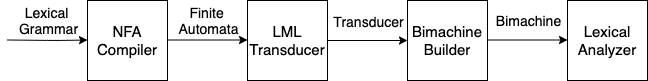
\includegraphics[
		width=14cm,
		keepaspectratio,
	  ]{img/architecture.png}
\end{figure}

В първата част ще представим разширен синтаксис на регулярен израз и разработка на recursive descent парсър, чрез който строим еквивалентния краен автомат. Във втората част ще разгледаме как се строи преобразувател от правила на заместване по стратегията най-ляво-най-дълго срещане и съответно как се строи бимашина по такъв преобразувател. Конструкцията на преобразувателя се съставя изцяло от операции над регулярни езици и релации. В третата част ще видим как се осъществява лексически анализ, чрез получената бимашина.

\subsection{От регулярен израз към краен автомат}

Регулярните изрази датират още от 50'те години на 20'ти век и са интегрирани в стандартните библиотеки на всички модерни езици за програмиране. Съществуват различни стандарти за представянето им, като тук ще ползваме синтаксис сходен с този на регулярните изрази в Perl. 
На Фигура \ref{fig:RegExSyntax} са представени базовите синтактични единици, чрез които конструираме регулярните изрази.

\begin{figure}[!htb]
	\begin{center}
		\begin{tabular}{ |l|l| } 
		\hline
		Израз & Пояснение \\
		\hline
		\verb/ab/ & конкатенация на символите 'a' и 'b' \\
		\verb/|/ & обединение (\verb/A|B/ - думата се разпознава от \verb/A/ или \verb/B/) \\
		\verb/*/ & 0 или повече срещания (Звезда на Килни) \\
		\verb/+/ & 1 или повече срещания \\
		\verb/?/ & 0 или 1 срещане \\
		\verb/./ & всеки символ от азбуката \\
		\verb/(...)/ & начало и край на група (разпознава израза в скобите) \\
		\verb/[...]/ & множество от символи (\verb/[0-9]/ разпознава цифрите от 0 до 9) \\
		\verb/[^...]/ & отрицание (разпознава символите, които не са в множеството) \\
		\verb/{n}/ & точно n на брой срещания \\
		\verb/{n,}/ & поне n на брой срещания \\
		\verb/{n,m}/ & от n до m на брой срещания \\
		\verb/\/ & буквална интерпретация на символ (\verb/\*/ разпознава '*') \\
		\hline
		\end{tabular}
	\end{center}
	\label{fig:RegExSyntax}
	\caption{Синтаксис на регулярен израз}
\end{figure}

\begin{example}
	Нека разгледаме няколко примерни регулярни израза спрямо описания синтаксис.
	\begin{itemize}
		\item \verb/(a|b)*c/ - разпознава думите, които се състоят от 0 или повече символи 'a' и 'b' и завършват на 'c' като на пример: \emph{ac, bc, abbabac, bbac, c, ...}
		\item \verb/.*true.*/ - думите, които съдържат "true": \emph{abctrue, 1true2_, true, ...}
		\item \verb/[a-zA-Z0-9@]+/ - разпознава думите, които се състоят единствено от латински букви, цифри и '@': \emph{z, 1b@, AbC123, 404, ccC, ...}
		\item \verb/[^ \t\r\n]/ - разпознава всички символи, които не са интервал, табулация или нов ред.
	\end{itemize}
\end{example}

За да построим краен автомат по регулярен израз е нужно първо да дефинираме граматическата му структура. Въвеждаме следната безконтекстна граматика на регулярен израз:

\begin{grammar}
	<expr> ::= <term>
	\alt <term> '|' <expr>

	<term> ::= <factor>
	\alt <factor> <term>

	<factor> ::= <atom>
	\alt <atom> <meta-char>
	\alt <atom> '\{' <char-count> '\}'

	<atom> ::= <char>
	\alt '.'
	\alt '(' <expr> ')'
	\alt '[' <char-class> ']'
	\alt '[' '\^{}' <char-class> ']'

	<char-class> ::= <char-class-item> 
	\alt <char-class-item> <char-class>

	<char-class-item> ::= <char> 
	\alt <char> '\-' <char>

	<char-count> ::= <integer> 
	\alt <integer> ',' 
	\alt <integer> ',' <integer>

	<integer> ::= <digit> 
	\alt <digit> <integer>

	<char> ::= \emph{anyCharExceptMeta}
	\alt '\textbackslash' <any-char>

	<any-char> ::= \emph{alphabet}

	<meta-char> ::= '?' \alt '*' \alt '+'

	<digit> ::= '0' | '1' | \dots | '9'
\end{grammar}

Следвайки тази граматика за всеки коректно дефиниран регулярен израз извличаме дърво на извод, по което чрез обхождане в дълбочина и строим недетерминиран краен автомат. Представяме автоматите и реализираме операциите по между им (конкатенация, обединение, звезда...) спрямо алгоритъма на Томпсън \cite{Thompson:68}. На Фигура \ref{parsetree} е изобразено дърво на извод на регулярен израз спрямо граматиката.

\begin{figure}
	\Tree[.\emph{expr} 
		[.\emph{term} 
		[.\emph{factor} 
			[.\emph{atom} 
				[( [.\emph{expr} 
					[
						[.\emph{term} [.\emph{factor} [.\emph{atom} [.\emph{char} a ]]]] 
						| 
						[.\emph{expr} [.\emph{term} [.\emph{factor} [.\emph{atom} [.\emph{char} b ]]]]  
					]]] 
				) ]]
			[.* ]]
		[.\emph{term}
			[.\emph{factor}
				[.\emph{atom}
					$[$
					[.\emph{char-class}
						[.\emph{char-class-item} [.\emph{char} 0 ] $-$ [.\emph{char} 9 ] ]]
					$]$ ]]]]]
	\label{parsetree}
	\caption{Дърво на извод за регулярния израз \texttt{(a|b)*[0-9]}, който разпознава думите, започващи с 0 или повече на брой символи 'a' и 'b', които завършват с цифра, на пример \emph{ab3, bbbb4, 9, aa1, baab4} и т.н. }
\end{figure}

Извличането на дърво на извод по зададен регулярен израз реализираме чрез \emph{рекурсивно спускане (recursive descent parser)}. Той спада към класа на типа парсъри, които строят дървото на извод \emph{"от горе надолу" (top-down)}, т.е. от корена към листата, започвайки от аксиомата на граматиката (нашия случай аксиомата е нетерминалът \emph{expr}). Граматически правила се прилагат от ляво на дясно. Регулярен израз е коректно дефиниран, ако по него може да се построи дърво на извод.

Особеност на \emph{top-down} парсърите е, че работят с ограничен клас от безконтекстни граматики. Ако граматиката съдържа \emph{лява рекурсия}, то е възможно процедурата да изпадне в безкраен цикъл поради факта, че правилата се прилагат от ляво на дясно. Нека разгледаме следния пример за директна рекурсия:

\[ A \to A \alpha \mid \beta \]

Символът \(A\) е нетерминал, докато \( \alpha \) и \( \beta \) са думи, съдържащи терминали и нетерминали, които обаче не започват с \(A\). Тъй като прилагаме правилата от ляво на дясно, то \(A\) ще опита първоначално да изведе \(A\) и така ще изпаднем в безкраен цикъл. Решението тук е да преобразуваме правилото до еквивалентната му дясно-рекурсивна форма.

\[ A \to \beta A' \]
\[ A' \to \alpha A' \mid \epsilon \]

Граматиката на регулярен израз не съдържа лява рекурсия, съответно можем по нея да реализираме \emph{recursive descent} парсър. Идеята е следната:

\begin{itemize}
	\item За всеки нетерминал (\emph{expr, term, factor...}) имплементираме отделен метод.
	\item Построяването на дървото започва с извикването на аксиомата на граматиката (\emph{Expr()}).
	\item Използваме методите \emph{Peek()}, за да видим следващия непрочетен символ от входа и \emph{Eat(char ch)}, който сравнява следващия следващия символ с \emph{ch} и преминава с една позиция напред. \emph{Next()} преминава към следващата позиция във входната дума без значение от символа, т.е. \emph{Eat(Peek())}.
\end{itemize}

Нека разгледаме реализацията на правилото за аксиомата на граматиката.

\begin{grammar}
	<expr> ::= <term>
	\alt <term> '|' <expr>
\end{grammar}

Нетерминалът \emph{expr} има два извода, като и двата започват с нетерминала \emph{term}. След като приложим правилото \emph{term}, проверяваме дали не сме стигнали до края на входа и в случай, че следващият символ е операторът за обединението, то местим входната дума с една позиция, прилагаме правилото \emph{expr} и връщаме обединението на резултатите.

\begin{lstlisting}[language=csh]
Fsa Expr() {
  var term = Term();
  if (HasMoreChars() && Peek() == '|') {
    Eat('|');
    return term.Union(Expr());
  }
  return term;
}
\end{lstlisting}

Важно е да уточним, че типът \verb/Fsa/ представлява краен автомат т.е. всеки метод, отговарящ на нетерминал в граматиката връща краен автомат. По този начин финалният автомат, съответстващ на регулярния израз се строи директно по време на получаването на дървото на извод. Нека разгледаме метода за нетерминала \emph{char}, който винаги извежда терминален символ, т.е. сме стигнали до листо на дървото.

\begin{lstlisting}[language=csh]
Fsa Char() {
  if (Peek() == '\') {
    Eat('\');
    var ch = Next();
    if (!alphabet.Contains(ch))
      throw new Exception($"Invalid char {ch}");
    return FsaBuilder.FromSymbol(ch);
  }	
  var ch = Next();
  if (metaChars.Contains(ch))
    throw new Exception($"Unescaped meta char {ch}");
  return FsaBuilder.FromSymbol(ch);
}
\end{lstlisting}

Ако сме стингали до символа '\textbackslash', последвалият го символ третираме като буква, независимо дали се използва като оператор. Методът връща автомат, който разпознава единствено прочетения символ.

\subsection{Конструкция на преобразувател по стратегията най-ляво-най-дълго срещане}

Алгоритъм за построяване на краен преобразувател по правила на заместване е представен от Каплан и Кей, 1994 \cite{Kaplan&Kay:94} и развит в последвалите разработки на Карттунен, 1996 \cite{Karttunen:96}, Гердеман и ван Ноорд, 1999 \cite{Gerdemann&VanNoord:99} и други. Базирайки се на тези статии, ще представим метод за имплементация на краен преобразувател по стратегията най-ляво-най-дълго срещане използвайки единствено алгебрата на регулярните езици и релации.

Дефинираме метода \emph{Fst ToLmlRewriter(Fst fst, ISet<char> alphabet)}, който по даден краен преобразувател и азбука, строи преобразувател по стратегията най-ляво-най-дълго срещане. Този метод извежда преобразувател, който представя релацията \( R^{LML}(T) \). Алгоритъмът се състои от четири стъпки като на всяка стъпка строим краен преобразувател и резултатът е композицията на тези преобразуватели в реда, в който са дефинирани.

\begin{enumerate}
	\item \emph{Първоначално срещане.} Строим преобразувател, който поставя маркер (\verb/cb/) в началото на всяко срещане на поддума (фокус) от входния текст, която е в домейна на входния преобразувател. Тази стъпка е ексивалентна на оператора \(AFTER\) и идентифицира всички контексти на заместване в текста независимо от това дали се застъпват, или са с възможно най-дълги фокуси. 
	\item \emph{От ляво на дясно.} Този преобразувател получава текста с маркерите от първата стъпка и поставя в началото и края на всеки контекст маркерите \verb/lb/ и \verb/rb/, като  \verb/cb/ се замества с \verb/lb/. Между маркерите за начало и край, не може да съществуват други маркери. Тази стъпка отговаря на оператора \(LEFTMOST\) и осигурява, че измежду контекстите със застъпващи се фокуси, ще останат тези с най-ляв фокус.
	\item \emph{Най-дълго-срещане}. Преобразувателят получава изхода от втората съпка и измежду маркираните контексти с еднакво начало, избира тези с най-дълъг фокус. Тази стъпка отговаря на оператора \(LONGEST\).
	\item \emph{Заместване.} В тази стъпка получаваме входния текст от стъпка 3, в който поддумите в домейна на преобразувателя са маркирани с \verb/lb/ и \verb/rb/ под стратегията най-ляво-най-дълго срещане. Този преобразувател извършва заместването на тези поддуми чрез входния преобразувател и премахва всички маркери.
\end{enumerate}

\begin{example}
	Имаме правилата на заместване \verb/ab+/ \( \to x \) и \verb/bc/ \( \to y \), съответстващи на релациите \( R_1, R_2 \). Входният преобразувател \(T\) представлява обединението: \( T := T_{R_1} \cup T_{R_2} \). Входният текст е \emph{abcabbdbc} и маркерите \verb/cb/, \verb/lb/ и \verb/rb/ представяме съответно чрез символите '!', '<' и '>'.
	\begin{enumerate}
		\item Маркираме началото на всички фокуси в думата: \emph{!a!bc!abbd!bc}
		\item Идентифицираме най-левите незастъпващи се контексти, което води до следните възможно декомпозиции: \emph{<ab>c<ab>bd<bc>} и \emph{<ab>c<abb>d<bc>}
		\item Прилагаме преобразвателят за най-дълго срещане и получаваме \emph{<ab>c<abb>d<bc>}
		\item Заместваме поддумите спрямо входния преобразувател и получаваме \emph{xcxdy}
	\end{enumerate}
\end{example}

За да имплементираме тези преобразуватели, първоначално дефинираме следните оператори спрямо Каплан и Кей \cite{Kaplan&Kay:94}:

...

\subsection{От краен преобразувател към бимашина}

\subsection{Лексически анализ чрез бимашина}

\pagebreak
\section{Алгоритми}

\pagebreak
\begin{thebibliography}{9}
	\bibitem{Kaplan&Kay:94} 
	Kaplan, Ronald and Kay, Martin. 1994.
	\textit{Regular models of phonological rule systems.}
	Computational Linguistics 20(3):331-378

	\bibitem{Gerdemann&VanNoord:99}
	Gerdemann, Dale and van Noord, Gertjan. 1999.
	\textit{Transducers from rewrite rules with backreferences}
	EACL '99: Proceedings of the ninth conference on European chapter of the Association for Computational Linguistics June 1999 Pages 126–133

	\bibitem{Karttunen:96}
	Karttunen, Lauri. 1996.
	\textit{Directed Replacement.}

	\bibitem{Schutzenberger:61} 
	Schützenberger, M.-P. 1961. 
	\textit{A remark on finite transducers.} 
	Information and Control, 4:185–196.

	\bibitem{Thompson:68} 
	Thompson, Ken 1968. 
	\textit{Regular Expression Search Algorithm.} 
	Association for Computing Machinery
	
\end{thebibliography}	

\end{document}
